\chapter{Dynamic Programming for Deterministic System}

\section{Deterministic Finite-State Problem}
%\subsection{Practical Difficulties of DP}
%\paragraph{The curse of dimensionality}
%(a) the \emph{exponential} growth of the computational and stoarge requirements as the number of state variables and control variables increases. 
%(b) Quick \emph{explosion} of the number of states in combinatorial problems
%(c) Intractability of the imperfect state information problems.
%\paragraph{The curse of modeling}
%It's hard to build 
%(a) mathematical models
%(b) computer / simulation models
%\paragraph{Practical constraints}
%The problem data may change as the system is controlled, and therefore online replanning is needed.
%
%
Consider a shortest path problem shown in Figure~(\ref{fig:2:1}).
\begin{figure}
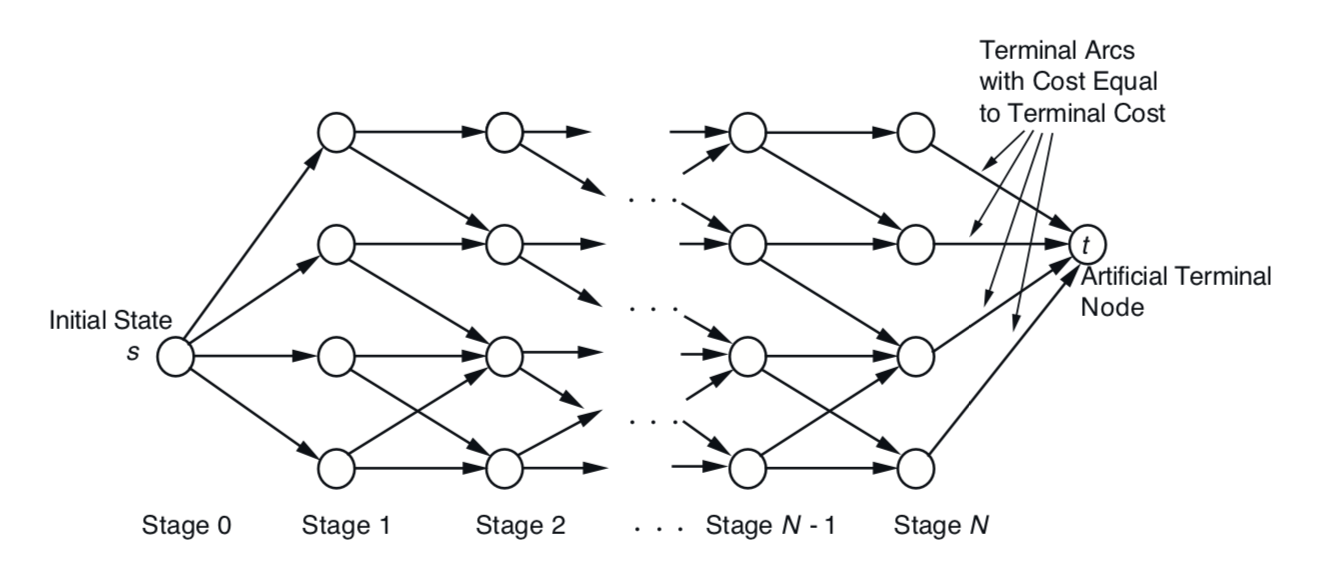
\includegraphics[width = 0.8\textwidth]{Second_lecture/p_1}
\caption{Illustration of shortest path problem}
\label{fig:2:1}
\end{figure}
We can convert the problem into a dynamic programming system as follows:
\begin{itemize}
\item
The states correspond to the nodes in each stage.
\item
The controls correspond to the acrs in each stage.
\item
The control sequences for this open-loop system correspond to paths from initial state to the terminal states.
\item
Let $a_{ij}^k$ denote the cost of transition (length of the arc) from the state $i\in S_k$ to state $j\in S_{k+1}$ at time $k$ 
\item
The cost of the control sequence is the cost of the corresponding path (total length of the path)
\end{itemize}
\paragraph{DP algorithms}
The backward algorithm applies as follows:
\begin{align*}
J_N(i)&=a_{ii}^N,\quad i\in S_N\\
J_k(i)&=\min_{j\in S_{k+1}}[a_{ij}^k + J_{k+1}(j)],\quad i\in S_k, k = N-1,N-2,\dots,0.
\end{align*}
Here the length of the shortest path from $s$ to $t$ equals to the $J_0(s)$. 

Note that the optimal path $s\to t$ is also an optimal path $t\to s$ for a \emph{reversed} shortest path problem, where the direction of each arc is reversed with its length unchanged.

Therefore, we can apply the backward DP algorithm for the reversed problem, which is so called the \emph{forward} DP algorithm:
\begin{align*}
\tilde{J}_N(j) &=a_{sj}^0,\quad j\in S_1,\\
\tilde{J}_k(j) &=\min_{i\in S_{N-k}}\left[
a_{ij}^{N-k} + \tilde{J}_{k+1}(i)
\right],\quad j\in S_{N-k+1}
\end{align*}
The optimal cost for the whole problem is $\tilde{J}_0(t) = \min_{i\in S_N}\left[a_{it}^N+\tilde{J}_1(i)\right]$.
The interpretation for this forward DP algorithm is that we can view $\tilde{J}_k(j)$ as the \emph{optimal cost-to-arrive} to state $j$ from initial state $s$.
\begin{remark}
There is no \emph{forward} DP algorithm for \emph{stochastic problems}.
This is becasue that we cannot restrict ourselves to open-loop sequences for the stochastic problems.
In other words, due to the uncertainty, the concept of \emph{optimal-cost-to-arrive} at the state $x_k$ does not make sense, i.e., it's impossible to guarantee (with probability 1) that any given state can be reached.

Fortunately, even for stochastic problems, the concept of \emph{optimal cost-to-go} from any state $x_k$ makes clear sense.
\end{remark}

\section{Generic Stochastic Path Problems}
Consider first a general deterministic shortest path($\bm s$) problems as follows:
\begin{itemize}
\item
Let $\{1,\dots,N,t\}$ denote the nodes of a graph, where $t$ is the destination.
\item
The $a_{ij}$ denotes the cost of moving from node $i$ to node $j$
\item
Our goal is to find a shortest (minimum cost) path from each node $i$ to node $t$
\item
Assumption: \emph{All cycles have non-negative} length, i.e., the optimal path \emph{need not take more than $N$ moves.}
\item
We can reformulate this problem as one where we require \emph{exactly} $N$ moves by allowing \emph{degerate moves} from a node $i$ to itself with cost $a_{ii}=0$. Moreover, we let
\begin{align*}
J_k(i)&=\emph{optimal cost of getting from $i$ to $t$ in $N-k$ moves}\\
J_0(i)&=\emph{cost of the optimal path from $i$ to $t$}
\end{align*}
\item
Therefore, we apply the DP algorithm as follows:
\[
\begin{array}{ll}
J_k(i)=\min_{j=1,\dots,N}\left[a_{ij} + J_{k+1}(j)\right],
&
k=0,1,\dots,N-2,
\end{array}
\]
with $J_{N-1}(i) = a_{it}, i=1,\dots,N$.
\end{itemize}

For example, consider the shortest paths problem shown in Fig~(\ref{fig:2:2}). Assume the destination node is the node $5$. The state $i$ means the current position is in the node $i$. In such case, note that
\begin{align*}
J_{N-1}(i)&=a_{it},\quad i=1,\dots,N\\
J_k(i)&=\min_{j=1,\dots,N}\left[a_{ij}+J_{k+1}(j)\right],\quad k=0,1,\dots,N-2
\end{align*}
The solution for this problem is shown in Fig.~(\ref{fig:2:2}b), where the arrow indicate the optimal move to node $5$ from the position at current stage.
\begin{figure}[H]
\centering
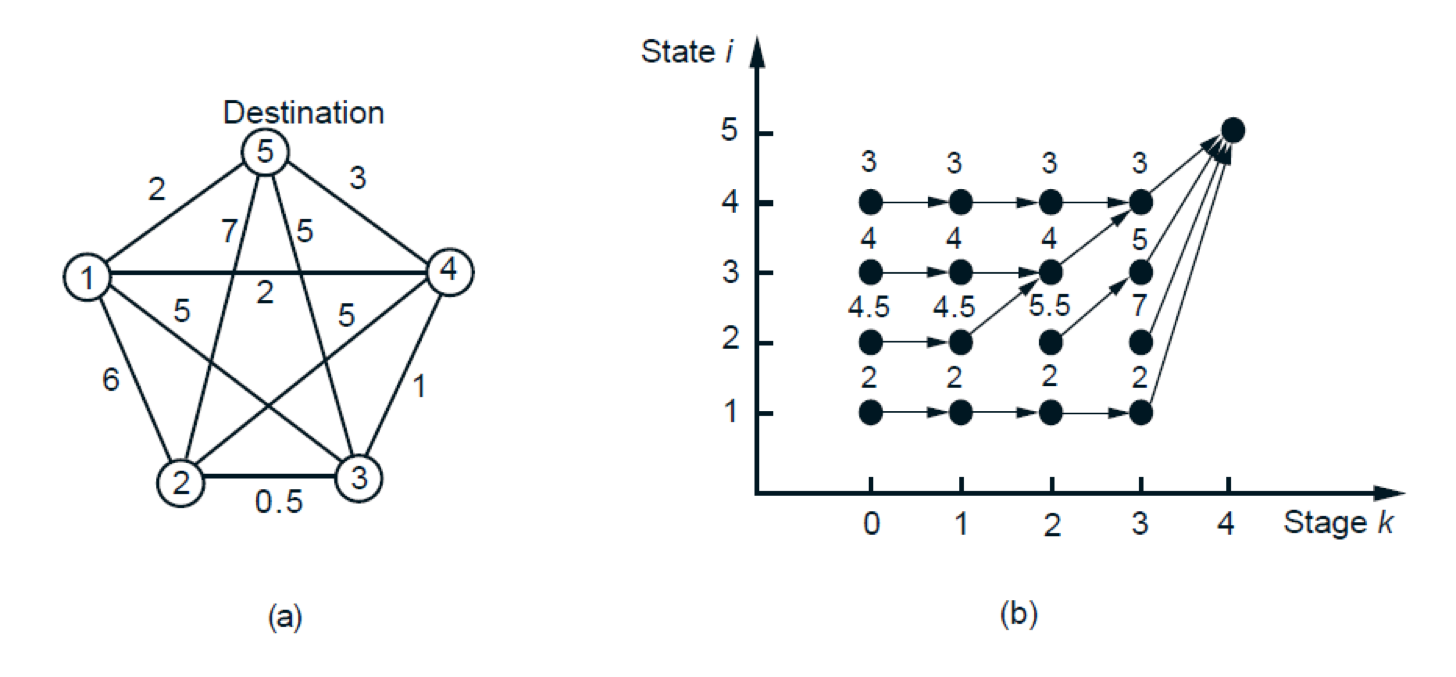
\includegraphics[width=0.8\textwidth]{Forth_lecture/p_1}
\caption{One Example of shortest paths problems}
\label{fig:2:2}
\end{figure}
\subsection{HMM setting and solving}
Now consider the \emph{Hidden Markov Models}. Suppose that the Markove chain is with transition probability $p_{ij}$, but the state transitions are hidden from our view. For each transition, we obtain an \emph{observation} instead. Let $r(z;i,j)$ denote the probability of observation taking value $z$ given the transition $i\to j$. The \emph{trajectory estimation problem} is that, given the observation sequence $Z_N=\{z_1,\dots,z_N\}$, what's the \emph{most likely} state transition sequence $\hat{X}_N:=\{\hat x_0,\hat x_1,\dots,\hat x_N\}$, i.e., the one equals to
\[
\arg\min_{\text{all }X_N}p(X_N\mid Z_N)=\frac{p(X_N,Z_N)}{p(Z_N)}
\]
We can rewrite the probability $p(X_N,Z_N)$ as follows:
\begin{align*}
p(X_N,Z_N)&:=p(x_{0:N},z_{1:N})\\
&=\pi_{x_0}\cdot p(x_{1:N},z_{1:N}\mid x_0)\\
&=\pi_{x_0}p(x_1,z_1\mid x_0)p(x_{2:N},z_{2:N}\mid x_{0:1},z_1)\\
&=\pi_{x_0}p_{x_0\to x_1}r(z_1;x_0,x_1)p(x_{2:N},z_{2:N}\mid x_{0:1},z_1)
\end{align*}
Following the similar idea, we compute
\begin{align*}
p(x_{2:N},z_{2:N}\mid x_{0:1},z_1)&=p(x_{2},z_2\mid x_{0:1},z_1)p(x_{3:N},z_{3:N}\mid x_{0:2},z_{1:2})\\
&=p_{x_1\to x_2}r(z_2;x_1,x_2)p(x_{3:N},z_{3:N}\mid x_{0:2},z_{1:2})
\end{align*}
Therefore, we derive
\[
p(X_N,Z_N)=\pi_{x_0}\prod_{k=1}^Np_{x_{k-1}\to x_k}
r(z_k;x_{k-1},x_k)
\]
Thus the problem is equivalent to
\[
\begin{array}{ll}
\mbox{minimize}
&
-\ln (\pi_{x_0})
-
\sum_{k=1}^N
\ln\left(p_{x_{k-1}\to x_k}
r(z_k;x_{k-1},x_k)
\right)
\end{array}
\]
over all possible sequences $\{x_0,x_1,\dots,x_N\}$. Therefore, due to the structure of our objective function, we can apply a distributed algorithm (e.g., dynamic programming) to solve it.

\section{General Shortest Path Algorithms}
Next, we discuss some non-DP shortest path algorithms. Note that they all can \emph{only} be used to solve deterministic finite-state problems.
The advantage is that they avoid computing the optimal cost-to-go for \emph{every} state.
This is essential for problems with \emph{huge} state spaces. (see examples in combinatorial optimization)

\subsection{Label Correcting Methods}
The idea of this kind of algorithm is to \emph{progressively} discover shorter paths from the origin to \emph{any other} node $i$, and to maintain the length of the shortest path found \emph{so far} in a variable $d_i$ (called the \emph{label} of $i$). 
\begin{itemize}
\item
If a shorter path to $i$ is found, then $d_i$ is reduced, and the algorithm checks if the labels $d_j$ can be reduced, where $j$ is the children of $i$, i.e., whether labels $d_j$'s can be reduced by setting them into $d_{i} + a_{ij}$.
\item
This algorithm makes use of a list of nodes called \emph{OPEN} (or \emph{candidate list}). This list contains nodes that are currently active such that they are candidates for further examination by the algorithm, and possible inclusion in the shortest path.

Initially, OPEN contains only $s$. Each node that has entered the OPEN at least once (except $s$) is assigned a \emph{parent} (refers to some node). The parent nodes are not necessary for the computation of shortest distance, but for tracing the shortest path to the origin after the algorithm terminates.
\end{itemize}
\paragraph{Notations}
\begin{itemize}
\item
$d_i$ denotes the \emph{label} of $i$, i.e., the length of the shortest path from $s$ to $i$ found so far. Initially $d_s=0,d_i=\infty,\forall i\ne s$
\item
UPPER: The label $d_t$ to the destination
\item
OPEN list: contains nodes that are currently active in the sense that they are candidates for further examination (initially OPEN = $\{s\}$)
\end{itemize}
The label correcting methods work as follows:

\begin{algorithm}[htb] 
\caption{The Label Correcting Methods} 
\label{alg:LCM} 
\begin{algorithmic}[1] %show number in each rows
\STATE \text{(Node Removal): }Remove a node $i$ from OPEN and for each child $j$ of $i$, do step 2
\STATE \textbf{(Node Insertion Test): }If $d_{i}+a_{ij}<\min\{d_j,\text{UPPER}\}$, set $d_j = d_j + a_{ij}$, and set $i$ to be the parent of $j$.
In additiion, if $j\ne t$, place $j$ into the OPEN if $j\notin\text{OPEN}$; 
otherwise set UPPER to the new value $d_i+a_{it}$ of $d_t$
\STATE\textbf{(Termination Test): }If OPEN is empty, terminate, else go to step 1. 
\label{code:GA}
\end{algorithmic}
\end{algorithm}
\begin{figure}
\centering
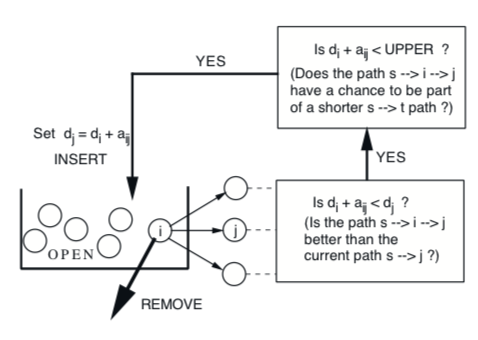
\includegraphics[width=0.8\textwidth]{Forth_lecture/p_2}
\caption{Diagram Illustration of Label Correcting Methods}
\end{figure}
Here we show how to apply the label correcting algorithm into the travelling salesman problem shown below.
\begin{figure}
\centering
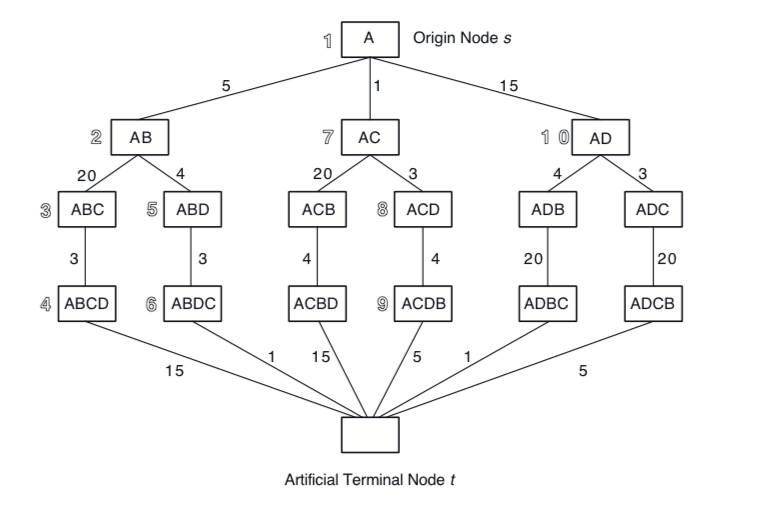
\includegraphics[width=0.8\textwidth]{Forth_lecture/p_5}
\caption{One example for travelling salesman problem}
\end{figure}
\[
\begin{array}{cccc}
\text{Iteation Number}&\text{Node Exiting OPEN}&\text{OPEN after Iteration}&\text{Upper}\\
0&-&1&\infty\\
1&1&2,7,10\\
2&2&3,5,7,10&\infty\\
3&3&4,5,7,10&\infty\\
4&4&5,7,10&43\\
5&5&6,7,10&43\\
6&6&7,10&13\\
7&7&8,10&13\\
8&8&9,10&13\\
9&9&10&13\\
10&10&\emptyset&13
\end{array}
\]
Note that some nodes never entered OPEN.

Finally, we give a verification for why label correcting methods work.
\begin{proposition}
If there exists at least one path from the origin to the destination, the label correcting algorithm terminates with UPPER equal to the shortest distance from the origin to the destination.
\end{proposition}
\begin{proof}
\begin{enumerate}
\item
Each time a node $j$ enters OPEN, its label is decreased and becomes equal to the length of some path from $i$ to $j$
\item
The number of possible distinct path lengths is finite, and therefore the number of timesa node can enter is finite, and the algorithm terminates.
\item
Let $\{(s,j_1,\dots,j_k,t),d^*\}$ be the pair of shortest path and the corresponding shortest distance.
If $\text{UPPER}>d^*$ at the termination, UPPER will also be larger than the length of all parths $(s,j_1,\dots,j_m), ,=1,\dots,k$ throguhout the algorithm, i.e., the node $j_k$ will never enter the OPEN list with $d_{j_k}$ equal to the shortest distance from $s$ to $j_k$.

Similarly, node $j_{k-1}$ will never enter to the OPEN list with $d_{j_{k-1}}$ equal to the shortest distance from $s$ to $j_{k-1}$. 
Continue to $j_1$ by induction will obtain a contradiction.
\end{enumerate}
\end{proof}
















